\documentclass[11pt, oneside]{article}   	% use "amsart" instead of "article" for AMSLaTeX format
\usepackage{geometry}                		% See geometry.pdf to learn the layout options. There are lots.
\geometry{letterpaper}                   		% ... or a4paper or a5paper or ... 
%\geometry{landscape}                		% Activate for for rotated page geometry
%\usepackage[parfill]{parskip}    		% Activate to begin paragraphs with an empty line rather than an indent
\usepackage{graphicx}				% Use pdf, png, jpg, or eps� with pdflatex; use eps in DVI mode
								% TeX will automatically convert eps --> pdf in pdflatex		
\usepackage{amssymb}
\usepackage{amsmath}
\usepackage{parskip}
\usepackage{url}

\title{Least squares and the mean}
%\author{The Author}
\date{}							% Activate to display a given date or no date

\graphicspath{{/Users/telliott_admin/Dropbox/Tex/png/}}

\begin{document}

\maketitle
%\section{}
% \subsection*{R code}
% \begin{lstlisting}  \end{lstlisting}
% \begin{center} 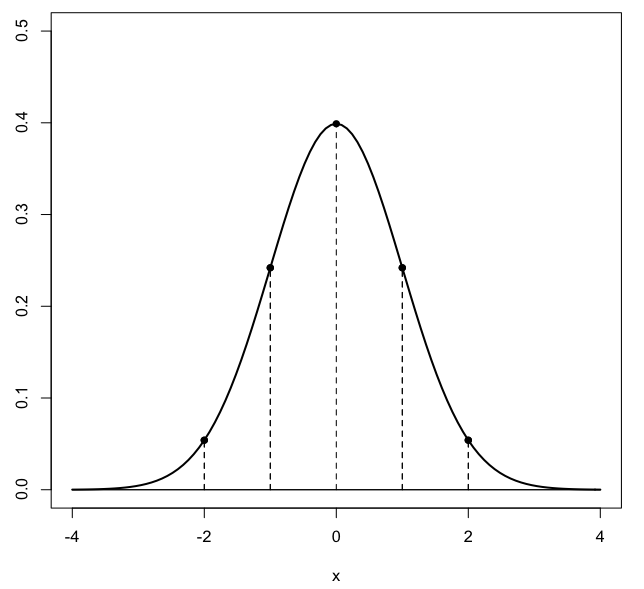
\includegraphics [scale=0.4] {gauss3.png} \end{center}
% \begin{bmatrix} a  &  b \\ c  &  d \end{bmatrix}
% \bigg |_

\Large

I found an interesting book free online, by D. Colquhoun (\emph{Lectures on Biostatistics}).  Here is a link to his website:

\url{http://www.dcscience.net}

and to a pdf of the book:

\url{http://www.dcscience.net/Lectures_on_biostatistics-ocr4.pdf}

On page 47 of the book, he says:

"The arithmetic mean of a sample is said to be a least squares estimate because the sum of the squares of the deviations from the arithmetic mean

\[ \sum (x_i - \bar{x})^2 \]

is smaller than the sum of the squares of the deviations from any other value.  This can be shown without using calculus."  Here is his derivation, rephrased only in part.

I like this problem because it's a very important result, but also because it provides some practice in thinking about summation.

Suppose that the sample consists of $N$ observations, $x_1, x_2, \dots, x_N$.  It is required to find a value of $m$ that makes $\sum (x_i - m)^2$ as small as possible.

This follows immediately from an algebraic identity which we will derive in a bit:

\[ \sum(x_i - m)^2 = \sum(x_i - \bar{x})^2 + N(\bar{x} - m)^2 \]

Clearly, for a given set of observations $x_i$, with mean $\bar{x}$, the minimum occurs when the second term is zero, that is, when  $\bar{x} = m$.  

We prove the identity as follows.  Recall that the definition of the arithmetic mean is $\bar{x} = \sum x_i / N$ so $N \bar{x} = \sum x_i$.  

Focusing our attention on the first term on the right-hand side above, we have

\[ \sum(x_i - \bar{x})^2 \]

expand by completing the square

\[ = \sum(x_i^2 - 2 x_i \bar{x} + \bar{x}^2)  \]
\[ = \sum x_i^2 - 2 \bar{x} \sum x_i + N \bar{x}^2 \]

Let's just stop and think about that second step for a minute.  First, we used the fact that the sum of a series of terms is the sum of the sums of the individual terms.  

Second, we can factor out constants from a sum, so that $\sum 2 x_i \bar{x} = 2 \bar{x} \sum x_i$ and $\sum \bar{x}^2 = \bar{x}^2 \sum 1$, where $\sum 1 = N$.  If this looks confusing, write the sum out more explicitly:

\[ \sum 1 = \sum_{i=1}^{i=N} 1 = N \]

Let's continue.  As we said, $N \bar{x} = \sum x_i$, so

\[ \sum x_i^2 - 2 \bar{x} \sum x_i + N \bar{x}^2 \]
\[ = \sum x_i^2 - 2 \bar{x} N \bar{x} + N \bar{x}^2 \]

Now we combinine this result with the completed square of the other part.  The entire right-hand side of our identity is:

\[ \sum x_i^2 - 2 \bar{x} N \bar{x} + N \bar{x}^2 + N(\bar{x}^2 - 2m \bar{x} + m^2) \]
\[ = \sum x_i^2 - 2 \bar{x} N \bar{x} + N \bar{x}^2 + N \bar{x}^2 - 2 Nm \bar{x} + Nm^2 \]

and (the whole point of this exercise), we can cancel all the terms in $\bar{x}^2$:

\[ = \sum x_i^2 - 2 Nm \bar{x} + Nm^2 \]

Now we need to go backward, and remove the factors of $N$ by reinstating the summation.  We have that 

\[ -2 N m \bar{x} = -2 m \bar{x} \sum 1 = - \sum 2 m \bar{x} \]

and similarly $N m^2 = \sum m^2$, so going back to what we had above:
\[ \sum x_i^2 - 2 Nm \bar{x} + Nm^2 \]
\[ = \sum x_i^2 - \sum 2 m \bar{x} + \sum m^2 \]
\[ = \sum (x_i^2 - 2 m \bar{x} +  m^2) \]
\[ = \sum(x_i - m)^2 \]

which is the left-hand side, above.

Alternatively and more elegantly, we can apply calculus to the problem of finding the value of $m$ that minimizes 
\[ \sum(x_i - m)^2 \]
\[ = \sum x_i^2 - 2m \sum x_i + Nm^2 \]

Keep in mind that the $x_i$ are \emph{constants} for a given sample, as are the sums of $x_i$ or $x_i^2$.  We differentiate with respect to $m$
\[ \frac{d}{dm} ( \sum x_i^2 - 2m \sum x_i + Nm^2) \]

The first term is zero.  The remaining terms give:
\[ = -2 \sum x_i + 2Nm \]

Set this equal to zero, as usual:
\[ 0 = -2 \sum x_i + 2Nm \]
\[ \sum x_i = Nm \]
\[ m = \frac{\sum x_i}{N} = \bar{x} \]

Sums can seem hard to reason about.  One approach that helps is to mentally expand the sum as 
\[ \sum x_i = x_1 + x_2 + \dots + x_N \]

and just reason using the normal rules of arithmetic.

Here are two other useful results dependent on manipulating sums.  The sum of the squares of the deviations from the mean is:

\[ \sum (x_i - \bar{x})^2 \]

It can be inconvenient to run through a list of values twice, once to find the mean and then again to do this calculation.  Expand the formula:

\[ \sum (x_i - \bar{x})^2 \]
\[ = \sum (x_i^2 - 2x_i \bar{x} + \bar{x}^2) \]
\[ = \sum x_i^2 - 2 \bar{x} \sum x_i + \bar{x}^2 \sum 1 \]

Since $\sum x_i = N \bar{x}$ and $\sum 1 = N$, we have that

\[ = \sum x_i^2 - 2  \bar{x} N \bar{x} + N \bar{x}^2 \]
\[ = \sum x_i^2 -  N \bar{x}^2 \]

and since $\bar{x} = \sum x_i / N$:

\[ \sum (x_i - \bar{x})^2 = \sum x_i^2 -  \frac{1}{N} \ (\sum x_i)^2 \]

Thus, to calculate the squared deviation, we form both the sum of the squared values and the sum of the values, squared. Then subtract $1/N$ times the latter from the former.

Just to check this with a simple example, suppose that we have the five numbers $1, 2, \dots 5$ with sum $1 + 2 + 3 + 4 + 5 = 15$ and mean equal to $3$.  Then the sum of the squared differences from the mean is $2^2 + 1^2 + 0^2 + 1^2 + 2^2 = 10$.

But the sum of the squared values is $1 + 4 + 9 + 16 + 25 = 55$.  The sum of the values, squared, is $15^2$, which when divided by $5$ is equal to $15 \times 3 = 45$ and then subtracted from $55$ is also equal to $10$.  It may seem harder the second way, but for a regular series there might be a shortcut using formulas like $n(n+1)/2$, etc.



In the same way, for a series of data points $(x_i,y_i)$, the covariance of $x$ with $y$ is defined as:

\[ Cov = \frac{1}{N-1} \sum(x_i - \bar{x})(y_i - \bar{y}) \]

We can expand the sum as

\[ = \sum(x_i y_i - x_i \bar{y} - y_i \bar{x} + \bar{x} \bar{y}) \]
\[ = \sum x_i y_i - \sum x_i \bar{y} - \sum y_i \bar{x} + \sum \bar{x} \bar{y}) \]

The individual terms on the right-hand side (after the first, neglecting the signs) are: 

\[ \sum x_i \bar{y} = \bar{y} \sum x_i = \frac{ \sum y_i}{N} \  \sum x_i \]
\[ \sum y_i \bar{x} = \bar{x} \sum y_i = \frac{ \sum x_i}{N} \  \sum y_i \]
\[ \sum \bar{x} \bar{y} = \bar{x} \bar{y} \sum 1 = \frac{ \sum x_i}{N} \ \frac{ \sum y_i}{N} \ N = \frac{ \sum x_i \sum y_i}{N} \]

Thus, each term is identical, except for sign, so we cancel two of them and obtain

\[ Cov = \frac{1}{N-1}  \sum x_i y_i - \frac{ \sum x_i \sum y_i}{N} \]

which is exactly as we had before in the case where $x_i = y_i$.  Covariance is defined such that the covariance of $x$ with $y$ is equal to the variance of $x$, in the case where $x_i = y_i$.

One other point to make before we stop.  Our original identity was:

\[ \sum(x_i - m)^2 = \sum(x_i - \bar{x})^2 + N(\bar{x} - m)^2 \]

This is true for any $m$, and in particular it holds where $\bar{x}$ is the mean of a \emph{sample} for a large population, and $\mu$ is the actual mean of the entire population, which is usually unknown and different than $\bar{x}$.  Then:

\[ \sum(x_i - \mu)^2 = \sum(x_i - \bar{x})^2 + N(\bar{x} - \mu)^2 \]

Multiply by $1/N$:

\[ \frac{ \sum(x_i - \mu)^2}{N} = \frac{\sum(x_i - \bar{x})^2}{N} + (\bar{x} - \mu)^2 \]

The left-hand side is the population variance, which is not necessarily equal to the sample variance.

There is more to say here, to give the reason for the $N-1$ form for sample variance.

\end{document}  